\chapter{Evaluation Methodology}%
\label{eval_method}

\section{Datasets}

The two agent types will be tested on two different sets of datasets.
These are the DeepMind mini-games, as well as the Simple64 map. These two
datasets should give an overall idea of how the agent is performing.

\subsection{Mini-games}

The mini-games consist of small, constrained challenges that represent
small parts of the full game of StarCraft II, allowing simple actions
in the game to be tested, as well as compared against a range of
published scores.

Every mini-game has a time limit, and the objective is to get the
highest score possible in the time frame. The scores for the game are surfaced
as part of the SC2LE \texttt{obs} object, meaning the agent is capable of easily
telling how well it is doing, and learning from this reward.

These mini-games are:

\begin{itemize}
    \item MoveToBeacon: A simple map with a single marine (player controlled
        unit) and a beacon, which acts as a target to move to. The agent gets
        a point each time it reaches the beacon, at which point the beacon's
        location is reset.
    \item CollectMineralShards: A map with two marines and 20 mineral shards,
        which act as items to pick up. Once all are picked up, 20 more are
        placed on the map. To achieve an optimum score, the two marines must
        be controlled independently, which results in this map being
        harder than the MoveToBeacon map.
    \item FindAndDefeatZerglings: A map with three marines and 25 zerglings,
        which are an enemy unit. A point is achieved for each zergling that
        is defeated, and a point lost any time a marine dies. This map
        is also the first to deal with the moving of the camera, as the previous
        two games had the entire state visible without moving the camera.
        Upon defeating the 25 zerglings, 25 more are added.
    \item DefeatRoaches: A map with nine marines and four roaches, which are a
        different enemy unit. This requires a more complex strategy to defeat,
        and also on defeating all four roaches, four more are spawned as well as 5
        more marines. This means the number of marines potentially grows
        throughout the game. However, a point is lost for any lost marines.
    \item DefeatZerglingsAndBanelings: A map with nine marines and six zerglings
        and four banelings. This again needs a different strategy and also gives
        extra marines upon defeating all the enemies.
    \item CollectMineralsAndGas: This map requires more strategy than the last.
        The map starts with 12 SCVs (which are gatherer units), a command centre
        (which is used to create additional units) and two types of collectable
        resources. The objective is to gather as many resources as possible, and
        also intelligently build more gathering units to increase the
        speed at which resources are gathered. An optimal strategy will also
        build an additional command centre.
    \item BuildMarines: This is the last and most complex map. The map starts
        with 12 SCVs, a command centre and eight resources to collect. The
        objective is to build as many marines as possible in the time limit.
        This requires the building of Supply Depots to store resources and
        barracks to build marines.
\end{itemize}

All of these mini-games have published scores for the many different
techniques as well as some baseline scores for human players and random
policies. This makes them ideal for testing a model again, such that the scores can
be directly compared.

\subsection{The \textbf{Simple64} Map}

\begin{figure}[h!]
    \centering
    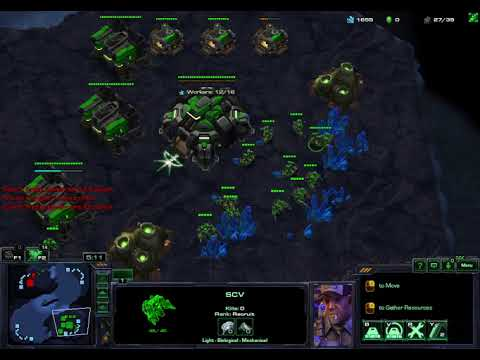
\includegraphics[width=1\textwidth]{simple64}
    \caption{Screen shot of the Simple64 map in-game.}%
    \label{fig:simple64}%
\end{figure}

The \textbf{Simple64} map was also chosen to allow experimentation on a
straightforward version of the full game, where the challenge is to beat the
games AI, which is built using more traditional game AI technology, and also can
cheat at higher difficulties.

The map contains a single opponent and two starting bases. The agent is spawned
into one of the two areas randomly and starts out with the \textbf{SCV} units,
characters for building and mining. The initial stage begins with mining of
necessary of resources for progressing through the level by creating the
required buildings and training \textbf{Marines}, fighter characters. This needs
the agent to control the \textbf{SCV} and \textbf{Marine} units using complex
three action commands. The end goal is to defeat the AI player and win the game.

One aspect that makes this much harder is the removal of a simple scoring
element, like that in the mini-games. This means the only scoring methods
available is the win/lose/draw score at the end of the game, of the ``Blizzard''
score that is given throughout, but is based on many different in-game aspects.
This makes it much harder for the agent to directly tell how well it is doing in
the global aspect of the game.

The more obvious element that makes this harder is that it combines all the
tasks that the mini-games cover, as well adding new tasks as the AI player will
attack bases and units, search and take resources, and build units and
buildings, all of which are not covered in the mini-games. This combination of
both new elements and a large number of already known elements makes the simple
64 maps much harder to play.

Due to this map containing a small snippet of the entire game, it will be useful
for measuring how the agent behaves in a general setting, as it is possible for
an agent to excel at each of the underlying tasks that go into a game of
StarCraft II, but to fail in the process of combining them effectively.

\section{Reasoning For Evaluation}

Evaluating the networks is essential for many reasons. Firstly, with the
mini-games the networks can be directly compared to both each other and also the
list of existing results, which is very useful for giving a direct metric for
the agents. Secondly, the Simple64 map is useful since it allows a lot of
interesting evaluations, both in the measuring of how the agent has generalised
from the individual tasks but also for how the agent does in a full game of
StarCraft II\@.

The accuracy of the agents is vital so that we can see if the agents have
started to learn the basics of the game. This is particularly easy as we can
rank how they perform against published results, to see if they rank higher than
random or straightforward agents, as well as comparing against the human
player's scores that are given. It is expected that both agents will perform
well and similar to each other for the first few mini-games before the more
complex ones should split them up further and show their inherent advantages and
disadvantages in their implementations. These compromises can then be compared,
to see which agent performs the best, and also to see what features of each
agent is the most desirable if a newer agent was to be built using the
information learnt from this project.

Generalisation is similarly crucial in that it allows us to see if an agent that
has learnt the basics of the game can then apply the lessons it has learnt to
situations that use the same skills but take place on a different map. This is
important for the agent, as it should be able to apply its skills regardless of
the map, like that of a human player. Furthermore, this is useful for giving
additional information on how the agent has learnt in the initial case. It is
possible the agent was able to learn some feature of the map at hand that
allowed it to do well in a mini-game, but when applied to a more realistic case,
the agent fails. Testing across new areas should allow this to be caught, as
well as giving an insight into how the agent would potentially fair if put on an
arbitrary map.

\section{Measuring Accuracy}

Firstly, we need to measure the accuracy of the agents, which requires us to
define what we mean by an accurate agent. The primary definition of saying how
accurate an agent is in taking an action will mostly depend on the final score
achieved through that episode. The game is being played in real-time and as so
creates complexity in the number of possible state action pairs that can be
observed. When the agent is playing in real-time, without any form of turn-based
playing, the state space is too large to represent using a tree structure of
all possible actions efficiently.

This means that when measuring the accuracy of an action, it will depend on the
final score. For example, the agent can go up or down and then go to the right
and attack an opponent on the square in-between. To achieve the same reward for
both actions, would mean that the optimal action to take could be either.

Broadly, what this means is that an accurate agent will be able to get a
competitive score in the mini-games, as due to their time limit, any actions
that are not needed would negatively impact its performance and in turn its
final score.

The main things that an agent must able to do are learn and improve. The learning
phase can be tested and shown by accumulating the loss function's value. These
values can then be analysed for a decline in values as more episodes are tested.
The loss function shows how far the policy's prediction was for a given action
and reward. As the agent trains, the predicted value and actual value should
converge. However, due to the random initialisation of each episode in a
mini-game, the process of identifying the correct sequence and pattern is
complicated since the agent will keep learning the wrong pattern. Because of this,
the loss function will never exactly converge to zero. This also keeps the
agent from over-fitting a single sequence of actions to take.

The final score of each episode is used to identify if the agent is learning the
correct actions to take. The agent should aim to maximise this value at all
times. When graphing the final score of multiple episodes, an increasing slope
will define the agent's performance with the training it had already done. If the
agent is learning and improving the policy, then the average of final scores
should increase. The average is used here due to the aforementioned random
differences in each run of the mini-games.

\begin{figure}[h!]
    \centering
    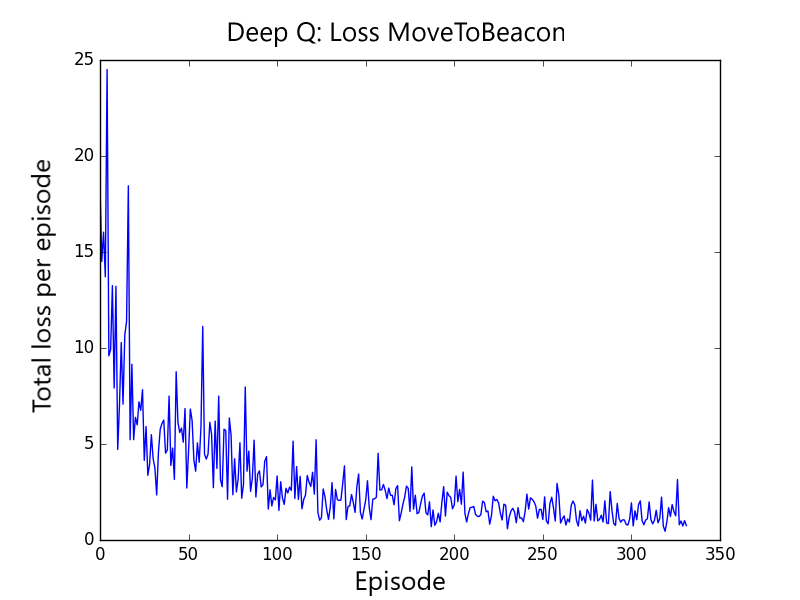
\includegraphics[width=1\textwidth]{loss_deepq_movetobeacon}
    \caption{Deep Q loss over 350 training episodes.}%
    \label{fig:loss_deepq_movetobeacon}%
\end{figure}


Figure~\ref{fig:loss_deepq_movetobeacon} shows the Deep Q agent's value
approximation converging to 0. The loss reduces to show the agent learning the
correct expected value.

\section{Measuring Generalisation}

Since the agent is being trained on a curriculum based system, the required
movements and actions the agent needs to take will be learnt on different
mini-games, each of which focuses on different skills. The agent will be trained
on different mini-games using the same model. So if a mini-game is focused on
moving to the beacon, the agent will learn the necessary state and action pairs
for achieving the highest score possible on that map. This allows the agent to
train on specific scenarios with a specified outcome. Ideally, training on one
of these scenarios should not affect the other actions that are not required.
However, there may be some overlap with the weights of the neural network being affected
by each given action. An agent could be learning on a mini-game that requires
it to attack. This would then reduce the weights of other non-attacking actions
such as building or moving.

To measure the agent's ability to generalise a given skill, the value of
a given policy will not work due to the issue of the agent reducing the value
policy of other actions. Instead, the agent's skill should apply to the
relevant field and tested on similar mechanics. So, an agent cannot be trained
on attacking and then tested on building. The agent should be tested on the same
actions but in different maps and scenarios.

However, the issue with training outside the mini-games is the
efficiency of a move comes into question. In the mini-games, sub-optimal actions
will lead to a lower score due to the time limits. However, when playing a
typical game of StarCraft II, even if on an easy map such as the Simple64 map,
this is not the case. The agent could take many sub-optimal actions, but still
be able to beat the in-game AI, and win the match. This makes it harder to
evaluate, as arguably an agent that performs lots of unneeded actions is not very
intelligent, but also if it can win, then it is not doing poorly. In the
end, the performance of the agent will need to be carefully monitored to ensure
that sub-optimal actions are only taken due to a lack of knowledge at that point
in the learning process, rather than thinking they are the most efficient
action.
